\newcommand*{\seancesection}[1]{%
  \addtocontents{toc}
  {\string\renewcommand\string\l@section{\string\@dottedtocline{1}{1.5em}{4.7em}}}
  \renewcommand*{\thesection}{Séance\space\arabic{section}}%
  \section{#1}
  \renewcommand*{\thesection}{\thechapter.\Alph{section}}%
  \addtocontents{toc}
  {\string\renewcommand\string\l@section{\string\@dottedtocline{1}{1.5em}{2.3em}}}
}
\newcommand{\Log}{\text{Log}}
\chapter{Analyse complexe : rappel TP}
\seancesection{Opérations sur les nombres complexes}
Soit $$ z=x+iy=re^{i\theta} \text{ avec }\left\{\begin{array}{l}
r=\sqrt{x^2+y^2}\\
\theta = sign(\text{Gauss})\arctan\left(\frac{y}{x}\right)
\end{array}\right.(\in\mathbb{R})$$
Formules de Moivre : $(\cos\theta+i\sin\theta)^n=\cos(n\theta)i\sin(n\theta)$\\
$z=\bar z\Rightarrow z\in\mathbb{R}$\\
$|z|=\sqrt{z\bar z}$

Pour les inégalités théoriques, si il y a des $|\dots|$ mettre au carré pour plus de racines et dev des 2 coté en parallèle. On trouvera la même chose à gauche et à droite à un facteur prêt, prouver l'inégalité sur les facteurs restants (ex2 a),b) )
$$Re(z)=\frac{z+\bar z}{2}\qquad Im(z)=\frac{z-\bar z}{2i}$$ $$\cos\theta=\frac{e^{i\theta}+e^{-i\theta}}{2}\qquad \sin\theta=\frac{e^{i\theta}-e^{-i\theta}}{2i}$$
$\cosh$ et $\sinh$ c'est pareil sans $i$.\\
$$z=0\Leftrightarrow \left\{\begin{array}{l}{Re}(z)=0\\ Im(z)=0\end{array}\right.$$
\seancesection{Limites, dérivabilité, Cauchy-Riemann}
Ne pas hésiter à utiliser Horner ou la division euclidienne.\\
Notion de différentielle en $z=z_0$ : 
$$\lim_{z_0}\frac{f(z)-f(z_0)}{z-z_0}$$
\newpage Équation Cauchy-Riemann : \begin{center}\fbox{\begin{minipage}{0.7\textwidth}
   Soit $f(z)=u(x,y)+i\,v(x,y)\ (u,v\in\mathbb{R})$, $f(z)$ est \textbf{différentiable} en $z=z_0$ si : $$\left\{\begin{array}{l}
   \partial_xu=\partial_yv\\
   \partial_yu=-\partial_xv
   \end{array}\right. \text{\Large{ ou }}\quad \partial_{\bar z}f(z)=0$$\\
   Calculé en $z=z_0$
   \end{minipage}}
\end{center}
La notion d'\textbf{analytique} en un point signifiant la différentiabilité de la fonction dans un voisinage du point (autour du point)


\seancesection{Fonctions usuelles}
Notion de dérivée : $$\lim_{|\Delta  z|\rightarrow 0} \frac{f(z_0+\Delta z)-f(z_0)}{\Delta z} $$
Quelques opérateurs : \begin{itemize}
\item $\log(z)=\ln|z|+i\,arg(z)$
\item $\Log(z) =\ln|z|+i\,Arg(z)\quad\text{où}\quad -\pi\leq Arg(z)\leq \pi$ 
\item $P(c,z) = e^{c\,\Log(z)}$
\end{itemize}
\paragraph{Remarque : } $\partial_z\Log(z)=\frac{1}{z}$. On ne peut pas utiliser la définition du logarithme pour la dérivation car $Arg(z)$ n'est pas rigoureusement indépendant de $z$.\\
Ici, le logarithme de base est de base \cancel{10} $e$.\\
$\Log(z)$ est analytique partout sur $\mathbb{C}\backslash\{z\leq 0\,|\,z\in\mathbb{R}\}$\\\\
\danger tout est a $2k\pi i$ prêt, c-a-d que si $z = 2$ c'est en réalité $z = 2e^{2k\pi i}$. Lors du passage de logarithme, ne pas oublier le $2k\pi i$
\seancesection{Analycité et intégrabilité. Intégrale de chemin}
Théorème de Cauchy-Goursat : \begin{center}\fbox{\begin{minipage}{0.7\textwidth}
   Soit $C$ un chemin admissible fermé simple. Soit $f(z)$ une fonction analytique en tout point de $C\cup D$ ($D$, domaine intérieur de $C$) $$\Rightarrow \oint_C f(z)\,dz=0$$
   \end{minipage}}
\end{center}
\newpage
Formule de Cauchy : \begin{center}\fbox{\begin{minipage}{0.7\textwidth}
   Soit $C$ un chemin admissible fermé simple. Soit $f(z)$ une fonction analytique en tout point de $C\cup D$ ($D$, domaine intérieur de $C$) et soit $z_0$ un point intérieur à $C$ ($z_0\in D$) $$\Rightarrow f^{(n)}(z_0) = \frac{n!}{2\pi i}\oint_C\frac{f(z)}{(z-z_0)^{n+1}}dz$$
    \end{minipage}}
\end{center}

\seancesection{}
Série de Taylor : \begin{center}\fbox{\begin{minipage}{0.7\textwidth}
   Si $f$ est analytique dans le \textbf{disque ouvert} $D$, $|z-z_0|<R$\\ Alors $\forall$ point $\in D$ $$f(z)=\sum_{n=0}^{\infty}a_n(z-z_0)^n\qquad|z-z_0|<R$$
   $$a_n = \frac{f^{(n)}(z_0)}{n!}\qquad n=0,1,2,\dots $$
    \end{minipage}}
\end{center}

Série de Laurent : \begin{center}\fbox{\begin{minipage}{0.7\textwidth}
   Si $f$ est analytique dans le \textbf{domaine} $D$, $R_1<|z-z_0|<R_2$\\
   $C$ un chemin admissible fermé entourant $z_0$ et $\in D$
    $$f(z)=\sum_{n=0}^\infty a_n(z-z_0)^n+\overbrace{\sum_{n=1}^\infty\frac{b_n}{(z-z_0)^n}}^{\text{partie principale}}\qquad R_1<|z-z_0|<R_2 $$ 
    $$ a_n = \frac{1}{2\pi i}\oint_C\frac{f(z)}{(z-z_0)^{n+1}}\,dz\quad ;\quad b_n=\frac{1}{2\pi i}\oint_C\frac{f(z)}{(z-z_0)^{1-n}}$$
    $$ (n=0,1,\dots) \qquad\quad\ ;\qquad (n=1,2,\dots)$$
    \end{minipage}}
\end{center}
Critère du Quotient : \begin{center}\fbox{\begin{minipage}{0.7\textwidth}
  Soit la série $\sum_0^\infty a_n$, la série converge ou diverge selon :
  $$\lim_{n\rightarrow\infty}\left|\frac{a_{n+1}}{a_n}\right|= \left\{\begin{array}{l}
<1 \rightarrow \text{ la série converge absolument}\\
= 1 \rightarrow\text{ on ne sait pas}\\
>1\rightarrow\text{ diverge} 
  \end{array}\right.$$
      \end{minipage}}
\end{center}
Important dans le TP $$\frac{1}{1-z}=\sum_{n=0}^\infty z^n\qquad (|z|<1)$$
On ne calculera quasi pas $a_n$ et $b_n$, il faut se débrouiller pour avoir quelque chose en $\frac{1}{(z-z_0)^n}$ et quelque chose en $(z-z_0)^n$ pour ainsi faire le lien avec Laurent.
\paragraph{Remarque } $|z-2|< 3 \Rightarrow 0<\frac{1}{|z-2|}<\frac{1}{3}$ et poser $u=\pm(z-2)$ pour alléger\\
Ne pas hésiter à passer par dérivation, ex : $\frac{1}{(z-1)^3}=-\frac{1}{2}\frac{d^2}{dz^2}\frac{1}{1-z}=-\frac{1}{2}\frac{d^2}{dz^2}\sum_0^\infty z^n$
\seancesection{Singularités, Séries de Laurent, Théorème des résidus}
\paragraph{Définition du résidus (en gros)} le résidu est le coefficient devant le terme en $\frac{1}{z-z_0}$ 	(étant dans la partie principale de la série de Laurent), $z_0$  étant le point singulier correspondant

Théorème des résidus : \begin{center}\fbox{\begin{minipage}{0.7\textwidth}
	Soit $C$ un chemin admissible fermé simple, orienté dans le sens positif et soit $f(z)$, analytique en tout point de $C\cup D$ sauf en un nombre fini de points singuliers isolés ($D$, intérieur de $C$)\\
	Soit $z_k$ ces points isolés $\in D$ $(k=1,\dots,n)$
	$$\Rightarrow \oint_Cf(z)\,dz=2\pi i\sum_{k=1}^n\underset{z=z_k}{\text{Res}}f(z)$$
      \end{minipage}}
      \end{center}
      
Théorème R1 : \begin{center}\fbox{\begin{minipage}{0.7\textwidth}
	Un point singulier isolé $z_0$ de $f(z)$ est un pôle d'ordre $m$ $$\Leftrightarrow f(z)=\frac{\Phi(z)}{(z-z_0)^m}\qquad\text{où}\quad\Phi(z)\text{ est analytique et non nulle en }z_0$$
	De plus $$\underset{z=z_0}{\text{Res}}f(z)=\Phi(z_0)\qquad\text{si }m=1$$
	$$\underset{z=z_0}{\text{Res}}f(z)=\frac{\Phi^{m-1}(z_0)}{(m-1)!}\qquad\text{si }m\geq 2$$
      \end{minipage}}
      \end{center}

Théorème R2 : \begin{center}\fbox{\begin{minipage}{0.7\textwidth}
	Soit 2 fonctions $p(z)$ et $q(z)$, analytique en $z_0$.\\ Si $\left\{\begin{array}{l	}
	p(z_0)\neq 0\\
	q(z_0)=0\text{ et }q'(z_0)\neq 0	
	\end{array}\right.$
	$\Rightarrow z_0$ est un pôle \textbf{simple} de $\frac{p(z)}{q(z)}$ et $$\underset{z=z_0}{\text{Res}}\frac{p(z)}{q(z)}=\frac{p(z_0)}{q'(z_0)}$$
      \end{minipage}}
      \end{center}    
Formule TP :  $$\underset{a}{\text{Res}}f(z)=\lim_{z\rightarrow a}\frac{\partial^{n-1}}{\partial z^{n-1}}((z-a)^nf(z))\qquad\text{où}\quad n:=\text{ordre de a}	 $$
Type particulier de point singulier :\begin{itemize}
\item éliminable :\begin{itemize}
\item "pôle d'ordre 0", la singularité se simplifie avec la racine du numérateur
\item la fonction n'existe pas en $z_0$ mais sa limite existe
\end{itemize}
\item essentiel :\begin{itemize}
\item "pôle d'ordre $\infty$", la partie principale a une infinité de termes
\end{itemize}
\end{itemize}
\seancesection{Applications du théorème des résidus}
 $$ P.V\int_{-\infty}^{+\infty}f(x)\,dx=\lim_{R\rightarrow\infty}\int_{-R}^R f(x)\, dx$$ où $P.V :=$ Valeur principale
 \paragraph{Propriété (pour $f(x)$ continue!)} \begin{itemize}
 \item Si $f(x)$ converge $(x\rightarrow\infty)\Rightarrow P.V\displaystyle\int\limits_{-\infty}^{+\infty}f(x)\,dx\ \exists$
 \item Si $f(x)$ est paire \textbf{et} $P.V\displaystyle\int\limits_{-\infty}^{+\infty}f(x)\,dx\ \exists$ $$\Rightarrow 2\int_0^{\infty}f(x)\,dx=\int_{-\infty}^{+\infty}f(x)\,dx=P.V\int_{-\infty}^{+\infty}d(x)\,dx$$
 \end{itemize}
Corollaire du Théorème des résidus : \begin{center}\fbox{\begin{minipage}{0.7\textwidth}
	Soit $C$ un chemin admissible fermé simple, orienté dans le sens positif et soit $f(z)$, analytique \textbf{sur $\mathbb{C}$} sauf en un nombre fini de points singuliers isolés \textbf{contenu à l'intérieur de $C$}\\
	$$\Rightarrow \oint_Cf(z)\,dz=2\pi i\underset{z=0}{\text{Res}}\left[\frac{1}{z^2}f\left(\frac{1}{z}\right)\right]$$
      \end{minipage}}
      \end{center}
\danger\ Ne pas se jeter tête baissée dans le corollaire, ou dans le théorème, erreur courante. Exemple de l'exo 1b (décomposition de la fraction en somme de fraction et prouver que la somme des résidus vaut 0, ce qui est beaucoup moins fastidieux, long et faisable que le théorème!)\\\\ 

Après avoir prouvé que $f(x)$ est borné et continue, on peut dire que $\displaystyle\int\limits_{-\infty}^{+\infty}$ équivaut à $\lim\limits_{R=\rightarrow\infty}\displaystyle\int\limits_{-R}^R$\\ 
De cela, on peut s'amuser... car en effet, on peut dire que (\autoref{fig::p}) $$\int_{-R}^R\dots+\int_{\gamma}\dots=\oint_C\dots$$ Il suffira donc de calculer l'intégrale sur le contour fermé (ce que l'on sait faire) et s'amuser avec celle sur la paramétrisation $\gamma$ (habituellement, on s'arrange pour qu'elle s'annule quand $R\rightarrow\infty$). Ainsi, on pourra déduire la valeur de l'intégrale de départ (bon exemple $\Rightarrow$ 2c et 3a)
\paragraph{Remarque} Si une des singularités se trouve sur la courbe $[-R,R]$, \textbf{il faut l'exclure}, comment? Au lieu de faire $2\pi i\text{ Res}$, ce sera $\pi i\text{ Res}$.\subparagraph{Explication} On mettait $2\pi i$ car en réalité, on contourne la singularité par un contour élémentaire pour l'exclure de notre contour (un cercle)$\Rightarrow 2\pi i$. Mais dans le cas d'une singularité sur le segment $[-R,R]$, pour exclure la singularité, il ne faut plus qu’un \textbf{demi}-cercle $\Rightarrow \pi i$
\begin{center}
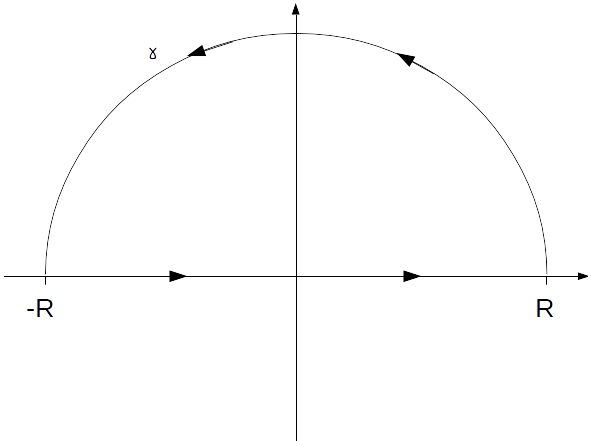
\includegraphics[scale=0.5]{test2}
\captionof{figure}{$R+\gamma=\text{O}$ dans le sens +}\label{fig::p}
\end{center}

\seancesection{Systèmes linéaires et permanents, produits de convolution, séries de Fourier}
2 type de système :\begin{itemize}
\item Système linéaire : \begin{itemize}
\item Propriété de superposition et d’homothétie
\item Pour le vérifier, poser $u(t)=au_1(t)+bu_2(t)$ et vérifier si $y(t) = ay_1(t)+by_2(t)$
\end{itemize}
\item Système permanent : \begin{itemize}
\item Si lorsque $y_0(t)$ est la sortie de $u_0(t)\Rightarrow y_0(t-t_0)$ est la sortie de $u_0(t-t_0)$
\item Pour le vérifier, poser $u(t)=u(t-t_0)$ et vérifier si $y(t)=y(t-t_0)$
\end{itemize}
\end{itemize}
Produit de convolution \begin{eqnarray}
y(t) &=& u(t)*h(t)=h(t)*u(t)\\
&=& \int_{-\infty}^{+\infty} u(\tau)\,h(t-\tau)\,d\tau\\
&=& \int_{-\infty}^{+\infty} h(\tau)\,u(t-\tau)\,d\tau
\end{eqnarray}
Propriété : $y(t)=y(t)*\underbrace{\delta(t)}_{\underset{\text{de Dirac}}{\text{Impulsion}}}$\\\\
Fonction de Heaviside : $$\nu(t)=\left\{\begin{array}{l}
0 \qquad \text{ si } t<0\\
1 \qquad \text{ si } t>0
\end{array}\right.$$ 
Série de Fourier d'un signal périodique \textbf{réel} $u(t)$ de période T
$$u(t)=\sum_{k=-\infty}^{+\infty}a_ke^{ik\omega_0t}$$ 
$$\text{ où }\qquad\omega_0=\frac{2\pi}{T},\qquad a_k=\frac{1}{T}\int_Tu(t)e^{-ik\omega_0t}\,dt $$
\paragraph{Remarque} Nous avons une exponentielle complexe dans l'intégrale, il est parfois judicieux de la décomposer en $\cos(k\omega_0t)$ et $\sin(k\omega_0t)$ pour faire apparaître les parités et ainsi, faire (parfois) plus simple\\
Petite précision sur $\delta(t-t_0)$, l'impulsion de Dirac : c'est une fonction nulle partout sauf en $t=t_0$ et dont la valeur est telle que la surface de l'impulsion $=1$\\
\danger\ Faire attention au changement de signe -\_-'
\seancesection{Transformées de Fourier et de Laplace	}
Petit rappel de Fourier (+notation supplémentaire) :
$$x(t)\overset{F}{\rightarrow}X(i\omega)=F(x(t))=\int_{-\infty}^{+\infty}x(t)\,e^{-i\omega t}\, dt $$
Nouveautés : $$X(i\omega)\overset{F^{-1}}{\rightarrow} x(t)=F^{-1}(X(i\omega))=\frac{1}{2\pi}\int_{-\infty}^{+\infty}X(i\omega)\,e^{i\omega t}\,d\omega$$
$$F\left(e^{i\omega_0t}\right) = 2\pi\delta(\omega-\omega_0)\qquad\text{car }F^{-1}(2\pi\delta(\omega-\omega_0)) = \frac{1}{2\pi}\int\dots=e^{i\omega_0t} $$
\paragraph{Remarque} $\omega_0\in\mathbb{R}$\\ \danger\ faire attention au \textbf{signe} et au \textbf{variable d'intégration}\\
Propriétés : 
$$x(t)\overset{F}{\underset{F^{-1}}{\rightleftharpoons}}X(i\omega)$$
\begin{alignat*}{4}
y(t) &= x(t-t_0) &&\overset{F}{\rightarrow} Y(i\omega)=e^{-i\omega t_0}X(i\omega)\\
y(t) &= e^{i\omega_0t}x(t) &&\
overset{F}{\rightarrow} Y(i\omega)=X(i(\omega-\omega_0))\\ 
y(t) &= x(at) &&\overset{F}{\rightarrow} Y(i\omega)=\frac{1}{|a|}X\left(i\frac{\omega}{a}\right)\qquad (a\in\mathbb{R}_0)\\
y(t) &= \frac{d}{dt}x(t) &&\overset{F}{\rightarrow} Y(i\omega)=i\omega X(i\omega)\\
y(t) &= -itx(t) &&\overset{F}{\rightarrow} Y(i\omega)=\frac{dX(i\omega)}{d\omega}
\end{alignat*}
$$\int_{-\infty}^{+\infty}|x(t)|^2\,dt=1\Leftrightarrow\int_{-\infty}{+\infty}|X(i\omega)|^2\,d\omega=2\pi $$
Transformation de Laplace : 
$$X(p)=\mathcal{L}(x(t))=\int_{-\infty}^{+\infty}x(t)\,e^{-pt}\,dt $$

\seancesection{Transformée de Laplace et équations différentielles}
\paragraph{Transformée de Laplace} \begin{align*}X(p) &=\mathcal{L}(x(t))=\int_{-\infty}^ {+\infty}x(t)e^ {-pt}\,dt\\
x(t) &= \frac{1}{2\pi i}\int_{\sigma-i\infty}^ {\sigma+i\infty}X(p)e^{pt}\,dp
\end{align*}
\subparagraph{Propriétés} \begin{alignat*}{5}
& y(t)=\overline{x(t)} &&\overset{\mathcal{L}}{\rightarrow} Y(p)=\overline{X(\bar{p})} & \alpha^+<\Re(p)<\alpha^-\\
& y(t)=x(t-t_0) &&\overset{\mathcal{L}}{\rightarrow} Y(p)=e^{-pt_0}X(p) & \alpha^+<\Re(p)<\alpha^- \\
& y(t)=e^{p_0t}x(t) &&\overset{\mathcal{L}}{\rightarrow} Y(p)= X(p-p_0) & \qquad\qquad\alpha^++\Re(p_0)<\Re(p)<\alpha^-+\Re(p_0)\\
& y(t)=x(at) &&\overset{\mathcal{L}}{\rightarrow} Y(p) = \frac{1}{|a|}X\left(\frac{p}{a}\right) & a\alpha^+<\Re(p)<a\alpha^-\\
& y(t)=\frac{d\,x(t)}{dt} &&\overset{\mathcal{L}}{\rightarrow} Y(p) =p\,X(p) & \alpha^+<\Re(p)<\alpha^-\\
& y(t)=-t\,x(t) &&\overset{\mathcal{L}}{\rightarrow}  Y(p)=\frac{d\,X(p)}{dp} & \alpha^+<\Re(p)<\alpha^-\\
& y(t)=\int_{-\infty}^t x(t)\,dt &&\overset{\mathcal{L}}{\rightarrow}  Y(p)=\frac{X(p)}{p} &  \alpha^+<\Re(p)<\alpha^-
\end{alignat*}
\paragraph{Inversion}
Les théorèmes (?) suivant utilisent la décomposition en fraction simple d'une fraction de polynômes.
\begin{center}\fbox{\begin{minipage}{0.7\textwidth}
	Soit $X(p)$, $\Re(p)>\alpha$, fraction avec $d^\circ_N<d^\circ_D$, si tous les pôles sont de multiplicité $=1$, on a $$X(p)=\sum_{i=1}^n\frac{\alpha_i}{p-\beta_i}\quad|\quad\Re(p)>\text{max}(\beta_i)$$ 
$$\Rightarrow x(t) = \sum_{i=1}^n\alpha_ie^{\beta_it}\nu(t)$$
      \end{minipage}}
      \end{center}
On comprendra que les $\alpha_i$ sont les coefficients trouvés en décomposant en fractions simples et que les $\beta_i$ sont les pôles.
\begin{center}\fbox{\begin{minipage}{0.7\textwidth}
	Soit $X(p)$ une fraction à coefficient réels, $\alpha^+<\Re(p)<\alpha^-$, soit $X(p)=X_g(p)+X_d(p)$ avec les pôles de $X_g$ (noté $p_g$) $\quad|\quad\Re(p_g)\leq\alpha^+$ et les pôles de $X_d$ (noté $p_d$) $\quad|\quad\Re(p_d)\geq\alpha^-$ $$\Rightarrow x(t)=\sum_{p\in p_g}\underset{p}{\text{Res }}[X_g(p)e^{pt}]\,\nu(t)-\sum_{p\in p_d}\underset{p}{\text{Res }}[X_d(p)e^{pt}]\,\nu(-t)$$
      \end{minipage}}
      \end{center}
\danger\ $\alpha^+$ est la borne inf, $\alpha^-$ est la borne sup\\
Le 2\up{ème} théorème est la généralisation du premier, il est important de réfléchir à quel pôle va se retrouver dans quelle partie ($X_g$ ou $X_d$) car en fonction de ça, il ne sera p-e pas nécessaire de tout décomposer en fraction simple.
\paragraph{Remarque} pour les fractions simples, il y a plus simple que de résoudre un système d'équation, soit : $$\frac{N(x)}{D(x)}=\frac{A}{x-x_1}+\frac{B}{x-x_2}+\frac{C}{x-x_3}+\dots$$ Pour trouver un coefficient, il suffit de reprendre la partie de gauche, la multiplier par le dénominateur du coefficient en question et de la calculer en la racine de ce dénominateur (le pôle de la fraction). Exemple pour A $$A=\left.\frac{N(x)}{D(x)}(x-x_1)\right|_{x=x_1}$$
la partie en $(x-x_1)$ va se simplifier avec une partie de $D(x)$ (logique) et on aura le résultat (cool non :D ).
\paragraph{Transformée $\mathcal{L}$ unilatérale}
$$X(p)=\text{$\mathbf{\mathcal{L}}$}_u(x(t))=\int_{0}^{\infty}x(t)e^{-pt}\,dt$$
\subparagraph{Propriétés}
$$\mathcal{L}_u\left(\frac{d^nx}{dt^n}\right)=p^nX_u(p)-p^{n-1}x(0^-)-p^{n-2}\frac{dx}{dt}(0^-)-\dots-\frac{d^{n-1}x}{dt^{n-1}}(0^-)$$
$$\Rightarrow \ddot{y}(t)=p^2Y_u(p)-py(0)-\dot y(0)\quad|\quad\dot y(t)=pY_u(p)-y(0)$$
\seancesection{Transmittances isomorphes et isochrones - Courbe de Bode}
Soit le système
$$e(t)\Longrightarrow \fbox{\quad h(t)\quad}\Longrightarrow v(t)$$
l'une des propriétés des transformées de Laplace est que convolution devient produit simple et vise versa.\\
Autrement dit, en prenant le système ci-dessus, on a : 
$$v(t)=e(t)*h(t)\Leftrightarrow V(p) = E(p)\,H(p)$$
\paragraph{Rappel} réponse $\left\{\begin{array}{ll}
\text{impulsionnellle} & h(t)\\
\text{indicielle} & S(t)
\end{array}\right.$. De plus,  $h(t)=\frac{dS(t)}{dt}$ et  $H(p)=pS(p)$\\

Après cela, on a les types de transmittance et de SLP
\begin{center}\fbox{\begin{minipage}{0.7\textwidth}
Transmittance isomorphe (= fonction de transfert)
$$H(p)=\left\{\begin{array}{ll}
\mathcal{L}(h(t)) & \text{T.L. de la réponse impulsionnelle}\\
\frac{V(p)}{E(p)} & \text{Rapport des T.L. d'entrée et de sortie}
\end{array}\right.$$
\end{minipage}}\end{center}
\begin{center}\fbox{\begin{minipage}{0.7\textwidth}
 \begin{align*}
\text{SLP stable} & \Leftrightarrow \text{"entrée bornée }\leftrightarrow\text{ sortie bornée"}\\
& \Leftrightarrow \int_{-\infty}^{+\infty}|h(T)|\,dT<+\infty
\end{align*}
\end{minipage}}\end{center}
\begin{center}\fbox{\begin{minipage}{0.7\textwidth}
\begin{align*}
\text{SLP stable} & \Rightarrow \text{RDC $H(p)$ contient $\Re(p)=0$ (que l'axe imaginaire)}\\
& \Rightarrow H(i\omega)\,\exists\text{ (tranmittance isochrone)}	
\end{align*}
\end{minipage}}\end{center}
\begin{center}\fbox{\begin{minipage}{0.7\textwidth}
SLP causal (demi-plan droit et impulsion nulle dans le passé) avec $H(p)$, fonction rationnelle
\begin{center}stable $\Leftrightarrow$ Tous les pôles $p_0$ de $H(p)$ ont $\Re(p)<0$\end{center}
\end{minipage}}\end{center}
Corollaire des théorèmes taubériens
\begin{center}\fbox{\begin{minipage}{0.7\textwidth}
Si $X(p)$ est fraction rationnelle avec \dots $$\Rightarrow\lim\limits_{t\rightarrow+\infty}x(t)=\lim\limits_{\sigma\rightarrow0^+}\sigma X(\sigma)$$
Si $X(p)$ est fraction rationnelle avec \dots $$\Rightarrow\lim\limits_{t\rightarrow 0^+}x(t) = \lim\limits_{\sigma\rightarrow +\infty}\sigma X(\sigma)$$
\end{minipage}}\end{center}